\documentclass{article}

% set font encoding for PDFLaTeX or XeLaTeX
\usepackage{ifxetex}
\ifxetex
  \usepackage{fontspec}
\else
  \usepackage[T1]{fontenc}
  \usepackage[utf8]{inputenc}
  \usepackage{lmodern}
  \usepackage{graphicx}
\fi

% used in maketitle
\title{Sondeo atmosferico}
\usepackage[left=3cm,right=3cm,top=3cm,bottom=3cm]{geometry}
\author{Luis Aarón Cerón Ramírez}
\date{02 de marzo del 2018}



% Enable SageTeX to run SageMath code right inside this LaTeX file.
% documentation: http://mirrors.ctan.org/macros/latex/contrib/sagetex/sagetexpackage.pdf
% \usepackage{sagetex}

\begin{document}
\maketitle
\section{Introducción}
Para poder estudiar si existe una situación atmosférica estable o inestable el conocimiento de la variación de la temperatura del aire con la altura resulta esencial. Dichos datos se miden a través de los radiosondeos y se representan en diagramas temperatura – altura. Estrictamente en dichos diagramas no se representa la temperatura frente a la altura expresada en metros, sino que ésta se representa frente a la presión, normalmente expresada en milibares. La presión atmosférica disminuye con la altura. Para una atmósfera estándar (representativa de los valores medios naturales) existe una correspondencia biunívoca entre la presión del aire y la altura. Aunque, desde este punto de vista, resulta formalmente equivalente la altura y la presión, esta última es una magnitud más útil para caracterizar el estado de la masa de aire y es más usada en cálculos termodinámicos.
\section{Fundamentos}
Un sondeo atmosférico es una medición de la distribución vertical de las propiedades físicas de la columna atmosférica, como presión, temperatura, velocidad del viento y dirección del viento (derivando así cizalladura del viento), contenido de agua líquida, concentración de ozono, contaminación y otras propiedades. Tales mediciones se realizan en una variedad de formas que incluyen detección remota y observaciones en el sitio.
El sonido in situ más común es una radiosonda, que generalmente es un globo meteorológico, pero también puede ser una sonda espacial.

Los sondeos de detección remota generalmente usan radiómetros infrarrojos y de microondas pasivos como instrumentos aerotransportados, estaciones de superficies, instrumentos satelitales de observación de la Tierra como AIRS y AMSU, observación de atmósferas en diferentes planetas, como la sonda de clima de Marte en el Mars Reconnaissance Orbiter.
\newline
Existen dos tipos de mediciones, la medición directa que consiste en sensores que miden los componentes atmosféricos directamente, como termómetros, barómetros y sensores de humedad, pueden enviarse en globos, cohetes o radiosondas. También pueden transportarse en los cascos exteriores de barcos y aviones o incluso montarse en torres. En este caso, todo lo que se necesita para capturar las mediciones son dispositivos de almacenamiento y/o transpondedores y el metodo indirecto que consiste en el caso más desafiante involucra sensores, principalmente montados en satélites, como radiómetros, sensores ópticos, radar, lidar y ceilómetro, así como de sodio, ya que estos no pueden medir la cantidad de interés, como temperatura, presión, humedad, etc., directamente. Al comprender los procesos de emisión y absorción, podemos descubrir qué está mirando el instrumento entre las capas de la atmósfera. Si bien este tipo de instrumento también se puede operar desde estaciones terrestres o vehículos -los métodos ópticos también se pueden usar dentro de instrumentos in situ- los instrumentos satelitales son particularmente importantes debido a su extensa y regular cobertura. Los instrumentos AMSU en tres NOAA y dos satélites EUMETSAT, por ejemplo, pueden muestrear todo el globo terráqueo a una resolución superior a un grado en menos de un día.
Podemos distinguir entre dos amplias clases de sensores: activos, como el radar, que tienen su propia fuente, y pasivos que solo detectan lo que ya está ahi.

\section{Analisis de datos}
Se analisaron los datos de la estación 71926 en baker lake Estados Unidos de America, en las fechas del 22 de junio y diciembre del 2017.

\section{Conclusion}
Como se puede bservar comparando las graficas, la de presion vs altura son graficas que tienen comportamientos muy parecidos, mientras que las demas graficas presentan comportamientos muy caoticos si las comparamos entre ellas, esto puede significar que no se tienen la misma cantidad de datos, ya que los lanzamientos pueden no realizarse con la misma frecuencia, o que las mediciones hayan variado demasiado un mes con respecto al otro, personalmente pienso que es esta ultima ya que son meses con estaciones diferentes, cosa que pienso yo puede afectar.

\section{Bibliografia}
Wikipedia contributors. (2017, March 5). Atmospheric sounding. In Wikipedia, The Free Encyclopedia. Retrieved 19:06, March 3, 2018

\section{Apendice}
¿Cuál es tu opinión general de esta actividad?
\newline
Es una actividad que ayuda a refuerza a utilizar jupyter notebook
\newline
¿Qué fue lo que más te agradó? ¿Lo que menos te agradó?
\newline
Lo que menos me agrado fue la elaboracion del reporte pues tuve demasiada dificultades con este, mientras qiue lo que mas me agrado fuel el hecho de utilizar jupyter para analizar datos.
\newline
¿Que consideras que aprendiste en esta actividad?
\newline
Utilizar un poco mas jupyter
\newline
¿Qué le faltó? ¿O le sobró?
\newline
me parecio que estab bien
\newline
¿Que mejoras sugieres a la actividad?
\newline
no tengo ninguna sugerencia


\section{Resultados}

Se comienza con las grafiicas obtenidas al a nalizar los datos de junio y diciembre
\begin{figure}[h]
  \centering
  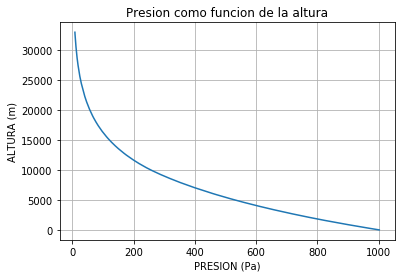
\includegraphics[scale=0.5]{presionj.png}
  \caption{Presion como funcion de la altura en junio }
\end{figure}

\begin{figure}[h]
  \centering
  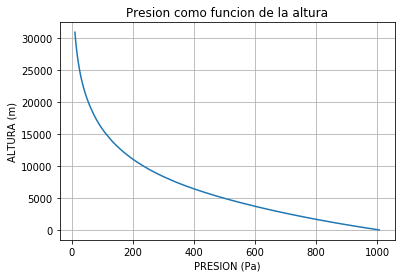
\includegraphics[scale=0.5]{presiond.png}
  \caption{Presion como funcion de la altura en diciembre}
\end{figure}


\begin{figure}[h]
  \centering
  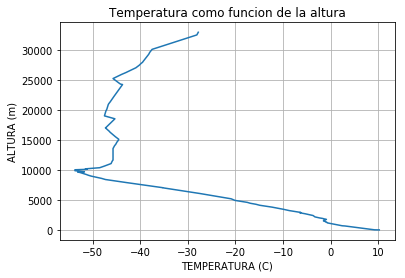
\includegraphics[scale=0.5]{tempj.png}
  \caption{Temperatura como funcion de la altura en junio }
\end{figure}

\begin{figure}
  \centering
  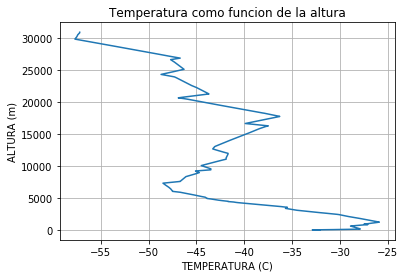
\includegraphics[scale=0.5]{tempd.png}
  \caption{Temperatura como funcion de la altura en diciembre }
\end{figure}


\begin{figure}[h]
  \centering
  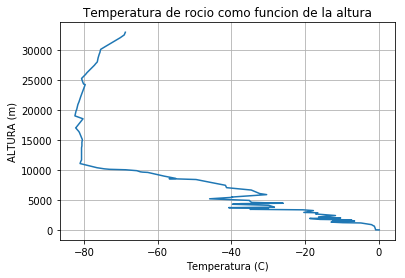
\includegraphics[scale=0.5]{rocioj.png}
  \caption{Temperatura del rocio como funcion de la altura en junio }
\end{figure}

\begin{figure}
  \centering
  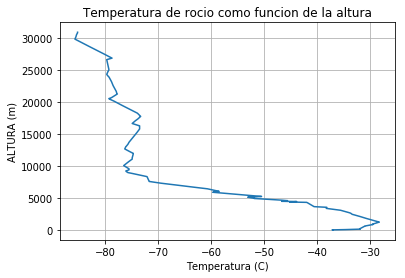
\includegraphics[scale=0.5]{rociod.png}
  \caption{Temperatura del rocio como funcion de la altura en diciembre }
\end{figure}


\begin{figure}[h]
  \centering
  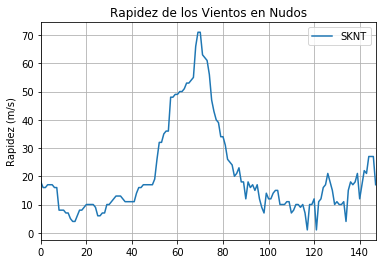
\includegraphics[scale=0.5]{nudosj.png}
  \caption{Rapidez de los vientos en nudos en el mes de junio}
\end{figure}

\begin{figure}
  \centering
  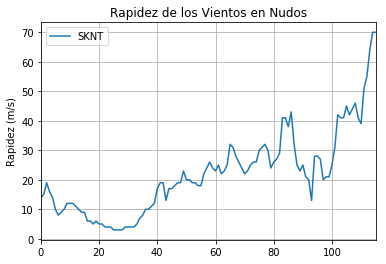
\includegraphics[scale=0.5]{nudosd.png}
  \caption{Rapidez de los vientos en nudos en el mes de diciembre}
\end{figure}

\begin{figure}[h]
  \centering
  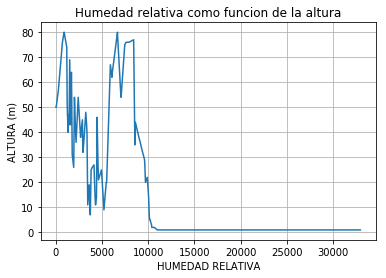
\includegraphics[scale=0.5]{humedadj.png}
  \caption{Humedad relativa como funcion de la altura del mes de junio}
\end{figure}

\begin{figure}[h!]
  \centering
  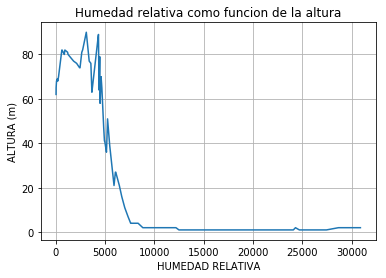
\includegraphics[scale=0.5]{humedadd.png}
  \caption{Humedad relativa como funcion de la altura del mes de diciembre}
\end{figure}




\end{document}

